	%% List of Packages to be included %%
%	\usepackage{tikz}
%	\usepackage{varwidth}
%	\usetikzlibrary{positioning}
%	\usetikzlibrary{calc}
	%% List of Packages to be included %%
	
  	%% modifier ici format police %%	
  	\setbeamerfont{title}{size=\Large}
	\setbeamerfont{frametitle}{size=\Large}
	\setbeamerfont{framesubtitle}{size=\scriptsize}
	\setbeamerfont{institute}{size=\scriptsize}
	\setbeamerfont{date}{size=\scriptsize}
	\setbeamerfont{author}{size=\normalsize}
	%% modifier ici format police %%


	\definecolor{MyColor}{rgb}{0.9297,0.5351,0.265312} 
	\newenvironment{changemargin}[2]{%  
	\begin{list}{}{%
			\setlength{\topsep}{0pt}%
			\setlength{\leftmargin}{#1}%
			\setlength{\rightmargin}{#2}%
			\setlength{\listparindent}{\parindent}%
			\setlength{\itemindent}{\parindent}%
			\setlength{\parsep}{\parskip}%
			\setlength{\topmargin}{-2cm}
		}%
		\item[]}{\end{list}
	}

\def\sizLRat{0.3}
\def\sizTRat{0.7}
\def\sizL2Rat{0.5}
\setbeamertemplate{title page}
{ 	\vspace{-0.5cm}
	\def\pp{0.79\paperwidth} 
	\begin{changemargin}{-1cm}{0cm}
		\begin{tikzpicture}
		\draw [anchor=north west](current page.north west) node  [inner sep=0pt] (pic) {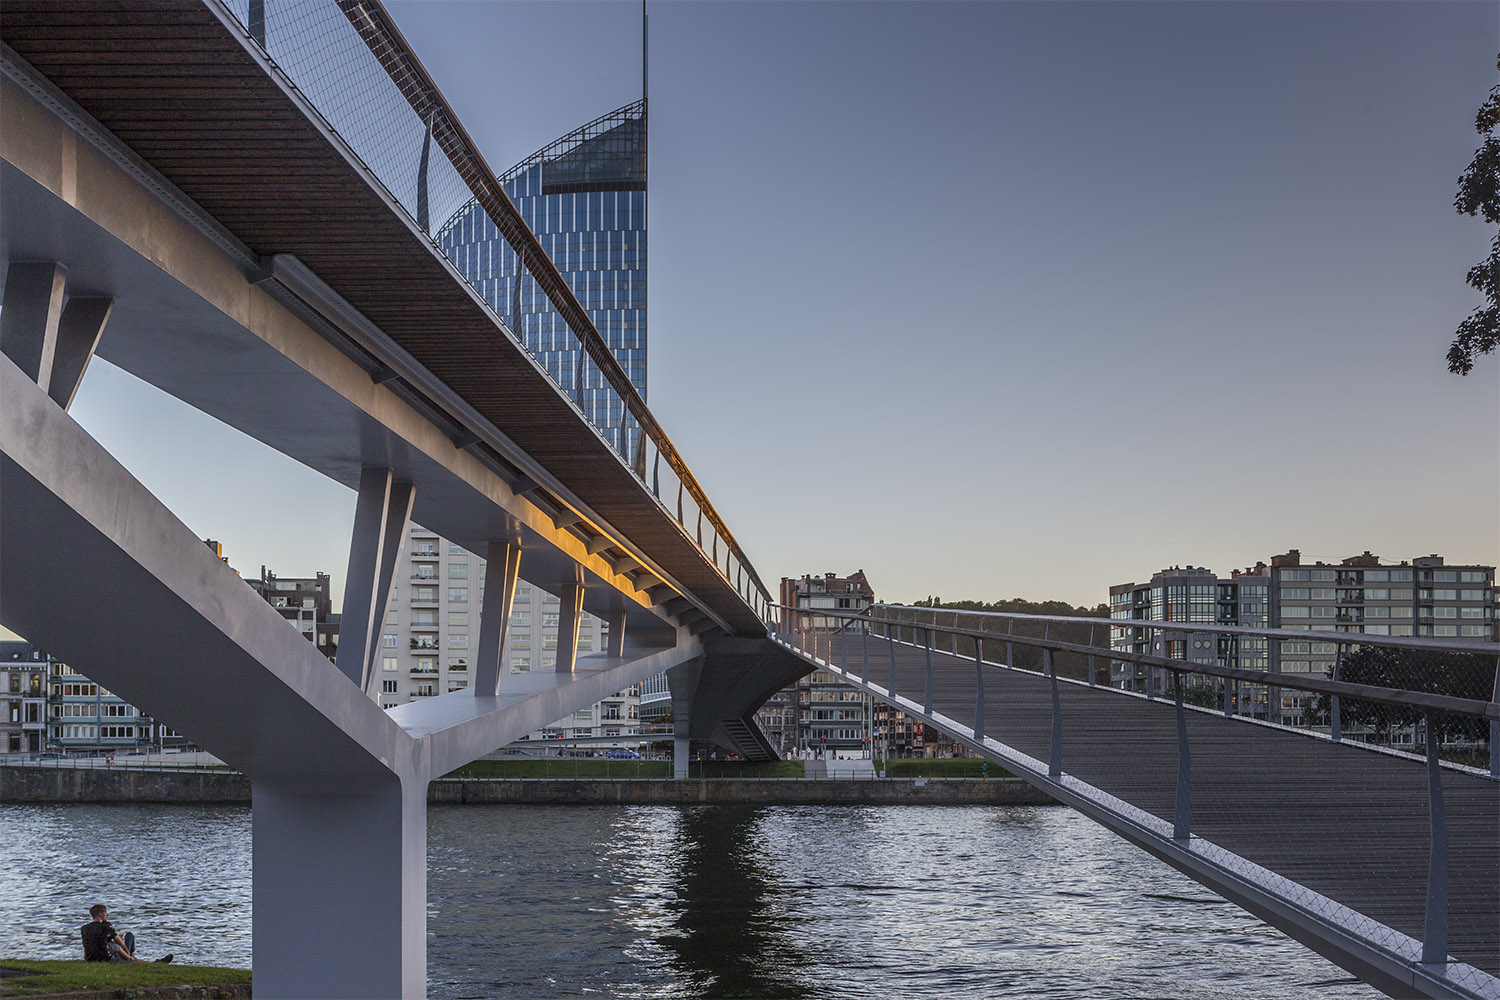
\includegraphics[width=\pp]{logos/image} } ;
		\coordinate (A) at (current page.south west) ;
		\coordinate (TL) at (current page.north west);
		\coordinate (D) at (current page.north east) ;
		\coordinate (E) at (current page.south east) ;
		\path (TL) --  coordinate [pos=\sizTRat] (B) (A) ;
		\path (TL) --  coordinate [pos=\sizTRat] (C) (D) ; 
		\fill [white] (A)--(B)--(C)--(D)--(E) ;
		\node[anchor=north east,xshift=-4pt,yshift=-4pt,align=right] at (current page.north east) {{
\includegraphics[width=0.25\paperwidth]{logos/facsa.pdf}}};
		\node[anchor=north east,xshift=-4pt,yshift=-35pt,align=right] at (D) {{
\includegraphics[width=0.37\paperwidth]{logos/logostocha} }};
		\node [anchor=north, text width=8cm, align=center,color=MyColor,minimum width=8cm] (titre) at (0.7\paperwidth,0.65\paperheight) {\usebeamerfont{title}\inserttitle\par} ;
		\node [anchor=north,below=0cm of titre,yshift=-15pt] (autr){\usebeamerfont{author}\insertauthor\par};
		\path (A) -- (TL) coordinate [pos=\sizL2Rat] (B') ;
		\path (A) -- (E) coordinate [pos=\sizTRat] (F) ;
		\fill [gray!10,fill opacity=0.8] (A) -- (B') -- (F) -- cycle ;
%		\node [inner sep=4pt,anchor=west] (conf)  at (0,0.1\paperheight) { \usebeamerfont{institute}\insertinstitute\par } ;
		\node [inner sep=5pt,anchor=south west,color=MyColor] (date) at (current page.south west) {\usebeamerfont{date}\insertdate\par }; 
		\node [anchor=west, inner sep=5pt,yshift=10pt,color=MyColor](date) at (0,0.05\paperheight) {\insertinstitute};
		\node [anchor=west,inner sep=20pt] at (0,0.22\paperheight) { \includegraphics[width=0.3\paperwidth]{\confLogo} };
		\node [anchor=south east,inner sep = 5pt] at (current page.south east) {{ 
\includegraphics[width=0.2\paperwidth]{logos/uee}}}  ;
		\end{tikzpicture}
	\end{changemargin}


}
 
 
\setbeamertemplate{frametitle}
{
	\vspace{0.3cm}\hspace{-0.8cm}
	\begin{tikzpicture}
	\node [color=MyColor,anchor=west] (A) at (0,0) {\begin{varwidth}{0.67\paperwidth} \bfseries \insertframetitle{} 	\end{varwidth}} ;
	\draw (A.south west) coordinate (B) [line width=0.6pt,color=MyColor]-- (A.south east);
	\draw [fill=MyColor, draw=MyColor] (B) circle(1.4pt) {};
	\coordinate (C) at (B.south west) ;
	\draw [anchor=west, color=MyColor] (B) node [yshift=-10pt] {\usebeamerfont{subtitle}\insertframesubtitle{}} ;
	\end{tikzpicture}
	\vspace{-0.2cm}
	\begin{tikzpicture}[remember picture,overlay]
	\node[anchor=north east,xshift=-4pt,yshift=-4pt] at (current page.north east) {
\includegraphics[width=0.25\paperwidth]{logos/facsa.pdf}};
%	\node [anchor=south east,inner sep = 5pt] at (current page.south east) {{ 
\includegraphics[width=0.2\paperwidth]{logos/uee}}}  ;
	\coordinate (A) at (current page.south west) ;
	\coordinate (TL) at (current page.north west);
	\coordinate (D) at (current page.north east) ;
	\coordinate (E) at (current page.south east) ;
	\path (A) -- (TL) coordinate [pos=\sizL2Rat] (B') ;
	\path (A) -- (E) coordinate [pos=\sizTRat] (F) ;
	\fill [gray!5,fill opacity=0.8] (A) -- (B') -- (F) -- cycle ;
	\node [anchor=south east,inner sep = 5pt,yshift=0pt] at (current page.south east) {\color{black}\scriptsize \insertframenumber{} /\inserttotalframenumber}  ;
	\node [anchor=south west] at (current page.south west) {\color{MyColor}\scriptsize \insertinstitute} ;
	\end{tikzpicture}
}

